\documentclass{article}
\usepackage{fancyhdr}
\usepackage{extramarks}
\usepackage{amsmath}
\usepackage{amsthm}
\usepackage{amsfonts}
\usepackage{tikz}
\usepackage[plain]{algorithm}
\usepackage{algpseudocode}

\begin{document}
\author{Chuan Lu}
\title{PHYS:5905 Homework 2}
\maketitle

\medskip

\begin{enumerate}

\item
Larmor Motion in constant, uniform magnetic field with zero electric field.

\begin{enumerate}
\item
Figure \ref{problem 1.1} shows the plots of $x(t)$, where the numerical solution is computed with $N=2000$ timesteps:
\begin{figure}[htbp]
\centering
\vbox{
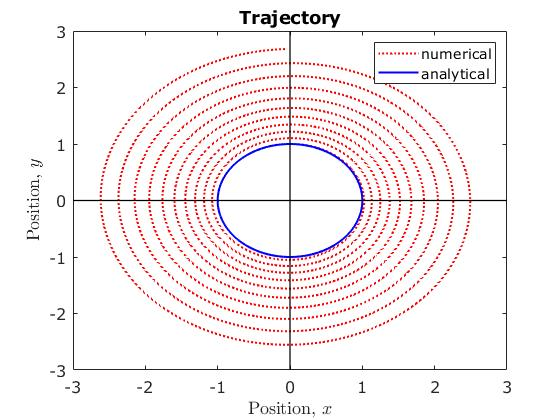
\includegraphics[scale=0.6]{problem1/trajectory_timestep_2000.jpg}
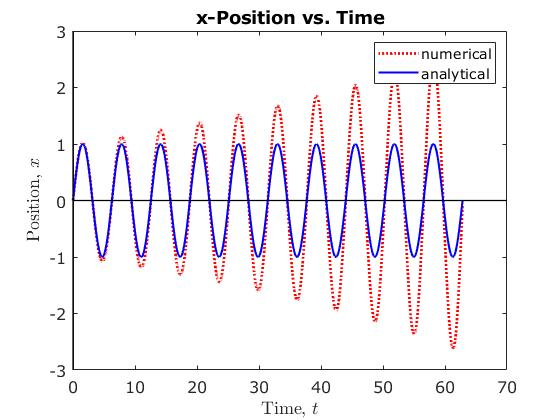
\includegraphics[scale=0.6]{problem1/xposition_timestep_2000.jpg}
}
\caption{The trajectory in the $(x, y)$ plane (top) and the position $x$ as function of time $t$ (bottom). The dot lines are numerical solutions solved with $N=2000$ timesteps and the solid lines are the analytical solutions.}
\label{problem 1.1}
\end{figure}

\item
Figure \ref{problem 1.2} is the error plot with respect to the number of timesteps. The slope is $k = -1.00393$.
\begin{figure}[htbp]
\centering
\vbox{
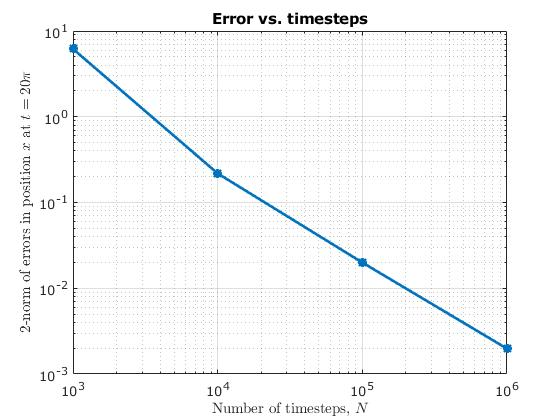
\includegraphics[scale=0.6]{problem1/error.jpg}
}
\caption{The error at $t = 20\pi$ with respect to the number of timesteps $N$.}
\label{problem 1.2}
\end{figure}

\end{enumerate}

\item
$E\times B$ drift in a constant, uniform magnetic and perpendicular electric field.

\begin{enumerate}
\item
Figure \ref{problem 2.1} shows the plots of $x(t)$, where the numerical solution is computed with $N=2000$ timesteps:
\begin{figure}[h]
\centering
\vbox{
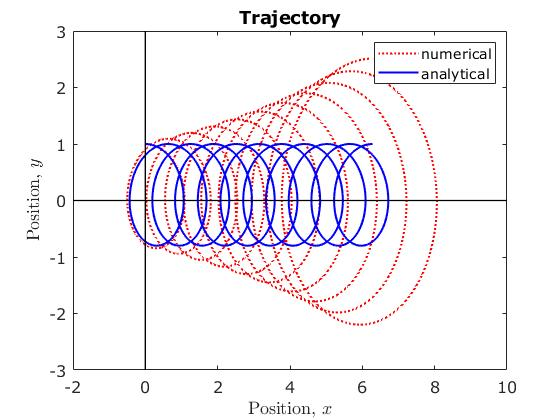
\includegraphics[scale=0.6]{problem2/trajectory_timestep_2000.jpg}
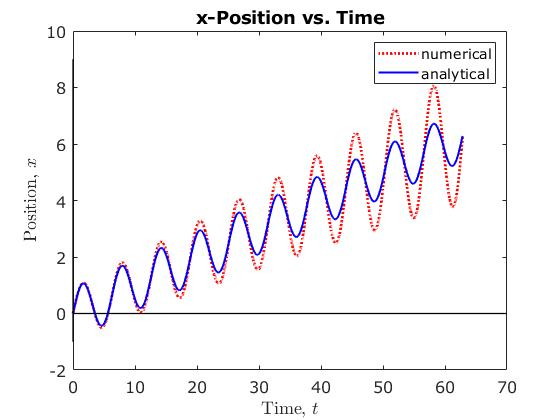
\includegraphics[scale=0.6]{problem2/xposition_timestep_2000.jpg}
}
\caption{The trajectory in the $(x, y)$ plane (top) and the position $x$ as function of time $t$ (bottom). The dot lines are numerical solutions solved with $N=2000$ timesteps and the solid lines are the analytical solutions.}
\label{problem 2.1}
\end{figure}

\item
Figure \ref{problem 2.2} is the error plot with respect to the number of timesteps. The slope is $k = -1.00389$.
\begin{figure}[h]
\centering
\vbox{
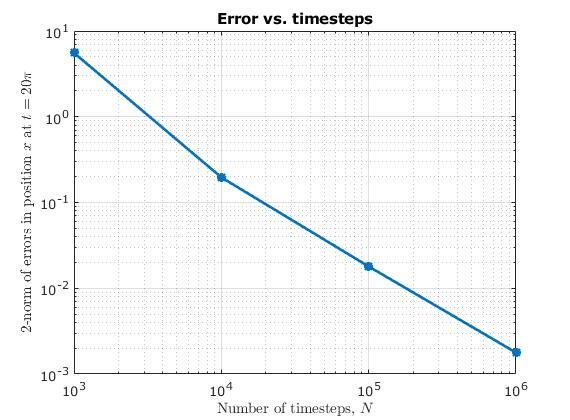
\includegraphics[scale=0.6]{problem2/error.jpg}
}
\caption{The error at $t = 20\pi$ with respect to the number of timesteps $N$.}
\label{problem 2.2}
\end{figure}

We notice that the slopes in both problems are just the same when the number of timesteps $N$ is large enough. This shows that the forward difference method is asymptotically linear.

\end{enumerate}

\end{enumerate}

\end{document}